\scanpage{19}
of the fibers $I_\alpha$ and $\widetilde A_\alpha$ of $I$ and $A$ over $\alpha$. The datum of a standard $G$-pinned curve over $\mathcal S$ is equivalent to the datum, \deleted{of} for \unsure{every|$\forall$} $\alpha\in S$, of a relative curve (proper smooth \inserted{relative\textsuperscript{ly}} $\unsure{6|0}$-connected) $Y_\alpha$ \unsure{over} $\mathcal S$, of relative genus $g_\alpha$, \uline{and} of an \inserted{$\mathcal S$-}monomorphism $(\widehat I_\alpha)_{\mathcal S}\hookrightarrow Y_\alpha$.

Let us denote, \deleted{by $\mathcal M_{g_\alpha,\deleted{\nu_\alpha}\inserted{\unsure{\widehat I_\alpha|\widehat I}}}$} for \deleted{\unsure{two|of}}\inserted{a} natural number $g\deleted{\unsure{\alpha|\nu}}$ and a finite set $I$ (of cardinality $\nu$) by
\figure{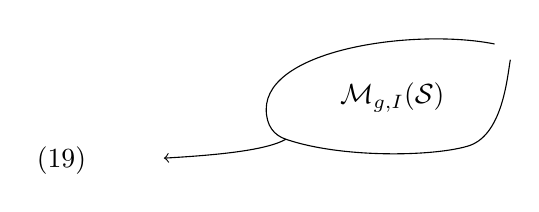
\begin{tikzpicture}[baseline=(m.base)]
\node (m) at (0,0) {$\mathcal M_{g,I}(\mathcal S)$};
\draw (1.3,.68) .. controls (.3,.88) and (-1.6,.62) .. (-1.6,-.15)
 .. controls (-1.6,-.36) and (-1.5,-.48) .. (-1.35,-.53)
 .. controls (-.65,-.77) and (.5,-.75) .. (.95,-.62)
 .. controls (1.4,-.5) and (1.46,.25) .. (1.5,.48);
\draw[->] (-1.35,-.53) .. controls (-1.6,-.67) and (-2.2,-.73) .. (-2.9,-.77);
\node at (-4.2,-.8) {$(19)$};
\end{tikzpicture}}
the \deleted{\unsure{category|category}}\inserted{groupoid} of relative curves $Y$ (proper, smooth, $0$-connected) over $\mathcal S$, \uline{$I$-pointed} i.e. equipped with a monomorphism $I_{\mathcal S}\hookrightarrow Y$. We thus find, if
\[
(20)\qquad\mathcal M_G(\mathcal S)
\]
denotes the groupoid of standard $G$-pinned curves over $\mathcal S$, an equivalence
\[
(21)\qquad\mathcal M_G(\mathcal S)\approxeq\prod_{\alpha\in S}\mathcal M_{g_\alpha,\widehat I_\alpha}(\mathcal S).
\]
\mspage{18}
